\documentclass[8pt]{beamer}

% Beamer style
%\usetheme[secheader]{Madrid}
% \usetheme{CambridgeUS}
\useoutertheme{infolines}
\usecolortheme[rgb={0.65,0.15,0.25}]{structure}
% \usefonttheme[onlymath]{serif}
\beamertemplatenavigationsymbolsempty
%\AtBeginSubsection

% Packages
%\usepackage[french]{babel}
\usepackage[latin1]{inputenc}
\usepackage{color}
\usepackage{xspace}
\usepackage{dsfont, stmaryrd}
\usepackage{amsmath, amsfonts, amssymb, stmaryrd}
\usepackage{epsfig}
\usepackage{tikz}
\usepackage{url}
% \usepackage{ulem}
\usepackage{/home/robin/LATEX/Biblio/astats}
%\usepackage[all]{xy}
\usepackage{graphicx}
\usepackage{xspace}

% Maths
% \newtheorem{theorem}{Theorem}
% \newtheorem{definition}{Definition}
\newtheorem{proposition}{Proposition}
% \newtheorem{assumption}{Assumption}
% \newtheorem{algorithm}{Algorithm}
% \newtheorem{lemma}{Lemma}
% \newtheorem{remark}{Remark}
% \newtheorem{exercise}{Exercise}
% \newcommand{\propname}{Prop.}
% \newcommand{\proof}{\noindent{\sl Proof:}\quad}
% \newcommand{\eproof}{$\blacksquare$}

% \setcounter{secnumdepth}{3}
% \setcounter{tocdepth}{3}
\newcommand{\pref}[1]{\ref{#1} p.\pageref{#1}}
\newcommand{\qref}[1]{\eqref{#1} p.\pageref{#1}}

% Colors : http://latexcolor.com/
\definecolor{darkred}{rgb}{0.65,0.15,0.25}
\definecolor{darkgreen}{rgb}{0,0.4,0}
\definecolor{darkred}{rgb}{0.65,0.15,0.25}
\definecolor{amethyst}{rgb}{0.6, 0.4, 0.8}
\definecolor{asparagus}{rgb}{0.53, 0.66, 0.42}
\definecolor{applegreen}{rgb}{0.55, 0.71, 0.0}
\definecolor{awesome}{rgb}{1.0, 0.13, 0.32}
\definecolor{blue-green}{rgb}{0.0, 0.87, 0.87}
\definecolor{red-ggplot}{rgb}{0.52, 0.25, 0.23}
\definecolor{green-ggplot}{rgb}{0.42, 0.58, 0.00}
\definecolor{purple-ggplot}{rgb}{0.34, 0.21, 0.44}
\definecolor{blue-ggplot}{rgb}{0.00, 0.49, 0.51}

% Commands
\newcommand{\backupbegin}{
   \newcounter{finalframe}
   \setcounter{finalframe}{\value{framenumber}}
}
\newcommand{\backupend}{
   \setcounter{framenumber}{\value{finalframe}}
}
\newcommand{\emphase}[1]{\textcolor{darkred}{#1}}
\newcommand{\comment}[1]{\textcolor{gray}{#1}}
\newcommand{\paragraph}[1]{\textcolor{darkred}{#1}}
\newcommand{\refer}[1]{{\small{\textcolor{gray}{{\cite{#1}}}}}}
\newcommand{\Refer}[1]{{\small{\textcolor{gray}{{[#1]}}}}}
\newcommand{\goto}[1]{{\small{\textcolor{blue}{[\#\ref{#1}]}}}}
\renewcommand{\newblock}{}

\newcommand{\tabequation}[1]{{\medskip \centerline{#1} \medskip}}
% \renewcommand{\binom}[2]{{\left(\begin{array}{c} #1 \\ #2 \end{array}\right)}}

% Variables 
\newcommand{\Abf}{{\bf A}}
\newcommand{\Beta}{\text{B}}
\newcommand{\Bcal}{\mathcal{B}}
\newcommand{\Bias}{\xspace\mathbb B}
\newcommand{\Cor}{{\mathbb C}\text{or}}
\newcommand{\Cov}{{\mathbb C}\text{ov}}
\newcommand{\cl}{\text{\it c}\ell}
\newcommand{\Ccal}{\mathcal{C}}
\newcommand{\cst}{\text{cst}}
\newcommand{\Dcal}{\mathcal{D}}
\newcommand{\Ecal}{\mathcal{E}}
\newcommand{\Esp}{\xspace\mathbb E}
\newcommand{\Espt}{\widetilde{\Esp}}
\newcommand{\Covt}{\widetilde{\Cov}}
\newcommand{\Ibb}{\mathbb I}
\newcommand{\Fcal}{\mathcal{F}}
\newcommand{\Gcal}{\mathcal{G}}
\newcommand{\Gam}{\mathcal{G}\text{am}}
\newcommand{\Hcal}{\mathcal{H}}
\newcommand{\Jcal}{\mathcal{J}}
\newcommand{\Lcal}{\mathcal{L}}
\newcommand{\Mt}{\widetilde{M}}
\newcommand{\mt}{\widetilde{m}}
\newcommand{\Nbb}{\mathbb{N}}
\newcommand{\Mcal}{\mathcal{M}}
\newcommand{\Ncal}{\mathcal{N}}
\newcommand{\Ocal}{\mathcal{O}}
\newcommand{\pt}{\widetilde{p}}
\newcommand{\Pt}{\widetilde{P}}
\newcommand{\Pbb}{\mathbb{P}}
\newcommand{\Pcal}{\mathcal{P}}
\newcommand{\Qcal}{\mathcal{Q}}
\newcommand{\qt}{\widetilde{q}}
\newcommand{\Rbb}{\mathbb{R}}
\newcommand{\Sbb}{\mathbb{S}}
\newcommand{\Scal}{\mathcal{S}}
\newcommand{\st}{\widetilde{s}}
\newcommand{\St}{\widetilde{S}}
\newcommand{\Tcal}{\mathcal{T}}
\newcommand{\todo}{\textcolor{red}{TO DO}}
\newcommand{\Ucal}{\mathcal{U}}
\newcommand{\Un}{\math{1}}
\newcommand{\Vcal}{\mathcal{V}}
\newcommand{\Var}{\mathbb V}
\newcommand{\Vart}{\widetilde{\Var}}
\newcommand{\Zcal}{\mathcal{Z}}

% Symboles & notations
\newcommand\independent{\protect\mathpalette{\protect\independenT}{\perp}}\def\independenT#1#2{\mathrel{\rlap{$#1#2$}\mkern2mu{#1#2}}} 
\renewcommand{\d}{\text{\xspace d}}
\newcommand{\gv}{\mid}
\newcommand{\ggv}{\, \| \, }
% \newcommand{\diag}{\text{diag}}
\newcommand{\card}[1]{\text{card}\left(#1\right)}
\newcommand{\trace}[1]{\text{tr}\left(#1\right)}
\newcommand{\matr}[1]{\boldsymbol{#1}}
\newcommand{\matrbf}[1]{\mathbf{#1}}
\newcommand{\vect}[1]{\matr{#1}} %% un peu inutile
\newcommand{\vectbf}[1]{\matrbf{#1}} %% un peu inutile
\newcommand{\trans}{\intercal}
\newcommand{\transpose}[1]{\matr{#1}^\trans}
\newcommand{\crossprod}[2]{\transpose{#1} \matr{#2}}
\newcommand{\tcrossprod}[2]{\matr{#1} \transpose{#2}}
\newcommand{\matprod}[2]{\matr{#1} \matr{#2}}
\DeclareMathOperator*{\argmin}{arg\,min}
\DeclareMathOperator*{\argmax}{arg\,max}
\DeclareMathOperator{\sign}{sign}
\DeclareMathOperator{\tr}{tr}
\newcommand{\ra}{\emphase{$\rightarrow$} \xspace}

% Hadamard, Kronecker and vec operators
\DeclareMathOperator{\Diag}{Diag} % matrix diagonal
\DeclareMathOperator{\diag}{diag} % vector diagonal
\DeclareMathOperator{\mtov}{vec} % matrix to vector
\newcommand{\kro}{\otimes} % Kronecker product
\newcommand{\had}{\odot}   % Hadamard product

% TikZ
\newcommand{\nodesize}{2em}
\newcommand{\edgeunit}{2.5*\nodesize}
\newcommand{\edgewidth}{1pt}
\tikzstyle{node}=[draw, circle, fill=black, minimum width=.75\nodesize, inner sep=0]
\tikzstyle{square}=[rectangle, draw]
\tikzstyle{param}=[draw, rectangle, fill=gray!50, minimum width=\nodesize, minimum height=\nodesize, inner sep=0]
\tikzstyle{hidden}=[draw, circle, fill=gray!50, minimum width=\nodesize, inner sep=0]
\tikzstyle{hiddenred}=[draw, circle, color=red, fill=gray!50, minimum width=\nodesize, inner sep=0]
\tikzstyle{observed}=[draw, circle, minimum width=\nodesize, inner sep=0]
\tikzstyle{observedred}=[draw, circle, minimum width=\nodesize, color=red, inner sep=0]
\tikzstyle{eliminated}=[draw, circle, minimum width=\nodesize, color=gray!50, inner sep=0]
\tikzstyle{empty}=[draw, circle, minimum width=\nodesize, color=white, inner sep=0]
\tikzstyle{blank}=[color=white]
\tikzstyle{nocircle}=[minimum width=\nodesize, inner sep=0]

\tikzstyle{edge}=[-, line width=\edgewidth]
\tikzstyle{edgebendleft}=[-, >=latex, line width=\edgewidth, bend left]
\tikzstyle{edgebendright}=[-, >=latex, line width=\edgewidth, bend right]
\tikzstyle{lightedge}=[-, line width=\edgewidth, color=gray!50]
\tikzstyle{lightedgebendleft}=[-, >=latex, line width=\edgewidth, bend left, color=gray!50]
\tikzstyle{lightedgebendright}=[-, >=latex, line width=\edgewidth, bend right, color=gray!50]
\tikzstyle{edgered}=[-, line width=\edgewidth, color=red]
\tikzstyle{edgebendleftred}=[-, >=latex, line width=\edgewidth, bend left, color=red]
\tikzstyle{edgebendrightred}=[-, >=latex, line width=\edgewidth, bend right, color=red]

\tikzstyle{arrow}=[->, >=latex, line width=\edgewidth]
\tikzstyle{arrowbendleft}=[->, >=latex, line width=\edgewidth, bend left]
\tikzstyle{arrowbendright}=[->, >=latex, line width=\edgewidth, bend right]
\tikzstyle{arrowred}=[->, >=latex, line width=\edgewidth, color=red]
\tikzstyle{arrowbendleftred}=[->, >=latex, line width=\edgewidth, bend left, color=red]
\tikzstyle{arrowbendrightred}=[->, >=latex, line width=\edgewidth, bend right, color=red]
\tikzstyle{arrowblue}=[->, >=latex, line width=\edgewidth, color=blue]
\tikzstyle{dashedarrow}=[->, >=latex, dashed, line width=\edgewidth]
\tikzstyle{dashededge}=[-, >=latex, dashed, line width=\edgewidth]
\tikzstyle{dashededgebendleft}=[-, >=latex, dashed, line width=\edgewidth, bend left]
\tikzstyle{lightarrow}=[->, >=latex, line width=\edgewidth, color=gray!50]

\newcommand{\GMSBM}{/home/robin/RECHERCHE/RESEAUX/EXPOSES/1903-SemStat/}
\newcommand{\figeconet}{/home/robin/RECHERCHE/ECOLOGIE/EXPOSES/1904-EcoNet-Lyon/Figs}
\newcommand{\fignet}{/home/robin/RECHERCHE/RESEAUX/EXPOSES/FIGURES}
\newcommand{\figeco}{/home/robin/RECHERCHE/ECOLOGIE/EXPOSES/FIGURES}
\newcommand{\figbayes}{/home/robin/RECHERCHE/BAYES/EXPOSES/FIGURES}
\newcommand{\figCMR}{/home/robin/Bureau/RECHERCHE/ECOLOGIE/CountPCA/sparsepca/Article/Network_JCGS/trunk/figs}
\newcommand{\figtree}{/home/robin/RECHERCHE/BAYES/VBEM-IS/VBEM-IS.git/Data/Tree/Fig}

\renewcommand{\nodesize}{1.75em}
\renewcommand{\edgeunit}{2.25*\nodesize}

%====================================================================
%====================================================================
\begin{document}
%====================================================================
%====================================================================
\title[PLN as a JSDM]{The Poisson log-normal model as a joint species distribution model}

\author[S. Robin]{S. Robin \\ ~\\
  {\small Sorbonne universit\'e, LPSM} \\ ~\\
  joint work with {\bf J. Chiquet}, {\bf M. Mariadassou} \\ ~\\ 
  + many others \\
  \nocite{CMR18a,CMR19,CMR20,CMR21}}

\date[CEBC, jun'25]{\small Centre d'Etudes Biologiques de Chiz\'e, jun'25}

\maketitle

%====================================================================
\frame{\frametitle{Outline} \tableofcontents}

%====================================================================
%====================================================================
\section{The Poisson log-normal model}
\frame{\frametitle{Outline} \tableofcontents[currentsection]}
%====================================================================
\subsection*{Joint species distribution models}
%====================================================================
\frame{\frametitle{Joint species distribution models} \pause

  \paragraph{Foreword.} 
  \begin{itemize}
    \setlength{\itemsep}{0.5\baselineskip}
    \item Not a specialist of microbiome
    \item Used to work on applications in bioinformatics, then microbial ecology, then (macroscopic?) ecology
    \item Examples borrowed from different fields
  \end{itemize}
  
  \pause \bigskip \bigskip
  \paragraph{Joint species distribution model (JSDM \refer{WBO15}):} aim at modelling the joint distribution of the abundance of a set of 'species' accounting for
  \begin{itemize}
    \setlength{\itemsep}{0.5\baselineskip}
    \item environmental (or experimental) conditions
    \item 'interactions' between species
    \item \textcolor{gray}{heterogeneity of the sampling protocole}
  \end{itemize}
}

%====================================================================
\frame{\frametitle{Typical example} \pause

  \begin{tabular}{cc}
    \hspace{-.04\textwidth}
    \begin{tabular}{p{.5\textwidth}}
      \paragraph{Fish species in Barents sea \refer{FNA06}:} 
      \begin{itemize}
       \item $89$ sites (stations), 
       \item $30$ fish species, 
       \item $4$ covariates
      \end{itemize}

      \bigskip \bigskip \bigskip 
      \paragraph{Questions:} 
      \begin{itemize}
        \item Do environmental conditions affect species abundances? (abiotic) \\~ 
        \item Do species abundances vary independently? (biotic)
      \end{itemize} 
    \end{tabular}
    &
    \begin{tabular}{p{.45\textwidth}}
      \paragraph{Abundance table $=Y$:} ~ \\
        {\footnotesize \begin{tabular}{rrrr}
        {\sl Hi.pl}\footnote{{\sl Hi.pl}: Long rough dab, {\sl An.lu}: Atlantic wolffish, {\sl Me.ae}: Haddock} & {\sl An.lu} & {\sl Me.ae} & \dots \\
%         \\ 
  %       Dab & Wolffish & Haddock \\ 
        \hline
        31  &   0  & 108 & \\
         4  &   0  & 110 & \\
        27  &   0  & 788 & \\
        13  &   0  & 295 & \\
        23  &   0  &  13 & \\
        20  &   0  &  97 & \\
        . & . & . & 
      \end{tabular}} 
      \\
      \bigskip 
      \bigskip 
      \paragraph{Environmental covariates $=X$:} ~ \\
        {\footnotesize \begin{tabular}{rrrr}
        Lat. & Long. & Depth & Temp. \\
        \hline
        71.10 & 22.43 & 349 & 3.95 \\
        71.32 & 23.68 & 382 & 3.75 \\
        71.60 & 24.90 & 294 & 3.45 \\
        71.27 & 25.88 & 304 & 3.65 \\
        71.52 & 28.12 & 384 & 3.35 \\
        71.48 & 29.10 & 344 & 3.65 \\
        . & . & . & .
      \end{tabular}}
      \bigskip
    \end{tabular}
  \end{tabular}
  
}

%====================================================================
\frame{\frametitle{Latent variable models}

  \bigskip
  \paragraph{Modelling the dependency.}
  \begin{itemize}
    \setlength{\itemsep}{0.5\baselineskip}
    \item Not always easy to propose a joint distribution for a set of dependent variables (abundances), especially when {\sl dealing with counts}.
    \item May resort to a set of unobserved (latent) variables to encode the dependency.
  \end{itemize}
  
  \pause \bigskip \bigskip 
  \paragraph{Some popular examples of latent variable models.}
  \begin{itemize}
    \setlength{\itemsep}{0.5\baselineskip}
    \item Mixed models (e.g. to account for parental structure in genetics)
    \item Principal component analysis (for dimension reduction)
    \item Hidden Markov models (for time series, genomic structure, ...)
  \end{itemize}
  
  
  \pause \bigskip \bigskip 
  \paragraph{Many (most?) joint species distribution models:} SpiecEasi \refer{KMM15}, HMSC \refer{OTN17}, gCoda \refer{FHZ17}, MRFcov \refer{CWL18}, ...
  
}

%====================================================================
\frame{\frametitle{The Poisson log-normal (PLN) model}

  \bigskip
  \paragraph{Data at hand} in each site (or sample)
  \begin{itemize}
    \setlength{\itemsep}{0.5\baselineskip}
    \item $Y_i =$ abundance vector for the $p$ species under study:
    $$
    Y_i = [Y_{i1} \; \dots \; Y_{ip}],
    $$
    \item $x_i =$ vector of environmental covariates (with dimension $d$):
    $$
    x_i = [x_{i1} \; \dots \; x_{id}].
    $$
  \end{itemize}

  \pause \bigskip \bigskip 
  \paragraph{PLN = latent variable model:} \refer{AiH89}
  \begin{itemize}
    \setlength{\itemsep}{0.5\baselineskip}
    \item A latent Gaussian vector $Z_i$ with covariance matrix $\Sigma$ is associated to each site $i$
    $$
    Z_i = [Z_{i1} \; \dots \; Z_{ip}] \sim \Ncal_p(0, \emphase{\Sigma}).
    $$
    \item The abundance $Y_{ij}$ of species $j$ in site $i$ depends on both the covariates and the corresponding latent $Z_{ij}$:
    $$
    Y_{ij} \textcolor{gray}{\; \mid Z_{ij}} \sim \Pcal\left(\exp(\mu_{ij})\right), 
    \qquad
    \mu_{ij} = \textcolor{gray}{o_{ij}\;+\;} x_i^\top \emphase{\beta_j} + Z_{ij}.
    $$
  \end{itemize}

}

%====================================================================
\frame{\frametitle{Interpretation of the parameters}
 
  \bigskip
  \begin{tabular}{cc}
    \hspace{-.04\textwidth}
    \begin{tabular}{p{.5\textwidth}}
      \paragraph{'Environmental' effects:} 
      $$
      \beta_{hj} = \text{effect of covariate $h$ on species $j$}
      $$
      \begin{itemize}
        \item $\beta = d \times p$ regression coefficient matrix, 
        \item 'abiotic' effects.
      \end{itemize}
      \bigskip ~
    \end{tabular}
    & \pause
    \begin{tabular}{p{.45\textwidth}}
      \includegraphics[width=.325\textwidth]{\figeco/BarentsFish-coeffAll}
    \end{tabular} 
    \\
    \begin{tabular}{p{.5\textwidth}} \pause
      \paragraph{Species 'interactions':} 
      $$
      \sigma_{jk} = \text{(latent) covariance between species $j$ and $k$}
      $$
      \begin{itemize}
        \item $\Sigma= p \times p$ (latent) covariance matrix,
        \item 'biotic interactions'.
      \end{itemize}
      \bigskip ~
    \end{tabular}
    & \pause
    \begin{tabular}{p{.45\textwidth}}
      \includegraphics[width=.325\textwidth]{\figeco/BarentsFish-corrAll} 
    \end{tabular}    
  \end{tabular}
 
}

%====================================================================
\frame{\frametitle{Distinguishing between environmental effects and species interactions}

  \pause
  \begin{tabular}{cc|c}
    \multicolumn{2}{l|}{\emphase{Barents fishes: Full model}} &
    \multicolumn{1}{l}{\onslide+<3>{\emphase{Null model}}} \\
    & & \\
    \multicolumn{2}{c|}{{$Y_{ij} \sim \Pcal(\exp(\emphase{x_i^\intercal \beta_j} + Z_{ij}))$}} &
    \multicolumn{1}{c}{{\onslide+<3>{$Y_{ij} \sim \Pcal(\exp(\emphase{\mu_j} + Z_{ij}))$}}} \\
    & & \\
    \multicolumn{2}{l|}{{$x_i =$ all covariates}} &
    \multicolumn{1}{l}{{\onslide+<3>{no covariate}}} \\ 
    & & \\
    & correlations between & \\
    inferred  correlations $\widehat{\Sigma}_{\text{full}}$ & 
    predictions: $x_i^\intercal \widehat{\beta}_j$ & 
    \onslide+<3>{inferred correlations $\widehat{\Sigma}_{\text{null}}$} \\ 
    \includegraphics[width=.3\textwidth, trim=20 20 20 20]{\figeco/BarentsFish-corrAll} 
    &
    \includegraphics[width=.3\textwidth, trim=20 20 20 20]{\figeco/BarentsFish-corrPred} &
    \onslide+<3>{\includegraphics[width=.3\textwidth, trim=20 20 20 20]{\figeco/BarentsFish-corrNull}}
  \end{tabular}

  }
%====================================================================
\frame{\frametitle{Some properties of the Poisson log-normal distribution}

  \pause \bigskip
  \paragraph{Overdispersion.} Due to the random effect $Z$
  \begin{align*}
    \Var(PLN) > \Var(\text{Poisson})
  \end{align*}
  
  \pause \bigskip \bigskip
  \paragraph{Latent correlations sign ($Z$) = observed correlation sign ($Y$).}
  $$
  \sign(\sigma_{jk}) = \sign(\Cor(Y_{ij}, Y_{ik})). 
  $$

  \pause \bigskip \bigskip
  \paragraph{Sampling effort.} Offset $o_{ij}$
  $$
  Y_{ij} 
  \sim \Pcal(\exp(o_{ij} + x_i^\intercal \beta_j + Z_{ij})) 
  = \Pcal(\emphase{e^{o_{ij}}} \exp(x_i^\intercal \beta_j + Z_{ij}))
  $$
  \begin{itemize}
    \item 'macroscopic' ecology: $o_{ij} =$ log-time of observation,
    \item metabarcoding: $o_{ij} =$ log-sequencing depth.
  \end{itemize}

  \pause \bigskip \bigskip
  \paragraph{Prediction.} Expected abundance:
  $\Esp(Y_{ij}) = \exp(x_i^\intercal \beta_j + \sigma_{jj}/2)$.

}



%====================================================================
%====================================================================
\section{Inference}
\frame{\frametitle{Outline} \tableofcontents[currentsection]}
%====================================================================
\subsection{Incomplete data models}
%====================================================================
\frame{\frametitle{Inference of incomplete data models} 

  \paragraph{Maximum likelihood inference.}
  $$
%   \widehat{\theta} = \arg
  \max_\theta \; \underset{\text{likelihood}}{\underbrace{p(Y; \theta)}}
  $$
  \ra No closed form for ${p(Y; \theta) = \int \underset{\text{complete likelihood}}{\underbrace{p(Y, Z; \theta)}} \d Z}$ in most latent variable models.

  \pause \bigskip \bigskip
  \paragraph{Incomplete data models.} EM algorithm \refer{DLR77}
  $$
  \theta^{h+1} = 
  \underset{\text{\normalsize \emphase{M step}}}{\underbrace{{\argmax}_\theta}} \;
  \underset{\text{\normalsize \emphase{E step}}}{\underbrace{\Esp_{\theta^h}}} \;
  [\log p(Y, Z; \theta) \mid Y)].
  $$
  
  \pause \bigskip \bigskip 
  \paragraph{E step = critical step:} Evaluate $p(Z \mid Y; \theta)$, i.e. \\
  \medskip
  \ra Retrieve sufficient information about the latent variables $Z$ based on the observed ones $Y$.
}

%====================================================================
\subsection*{Variational approximation}
%====================================================================
\frame{\frametitle{Case of the Poisson log-normal model} 

  \bigskip
  \paragraph{Intractable E step.} No reasonably easy way to compute $p(Z_i | Y_i; \theta)$ under PLN.

  \pause \bigskip \bigskip
  \paragraph{Twisted problem.} Approximate it with some other (nice) distribution, e.g.
  $$
  p(Z_i | Y_i; \theta) \simeq \Ncal(m_i, S_i).
  $$
  \begin{itemize}
    \setlength{\itemsep}{0.5\baselineskip}
    \item Variational approximation \refer{WaJ08,BKM17} ('E' step $\to$ 'VE' step).
    \item Computationaly efficient (can deal with $\simeq 10^3$ samples or species).
  \end{itemize}
  
  \pause \bigskip \bigskip
  \paragraph{But...} 
  \begin{itemize}
    \setlength{\itemsep}{0.5\baselineskip}
    \item $\neq$ Maximum likelihood
    \item Very few statistical guaranty (consistency, asymptotic normality, asymptotic variance, ...).
    \item No direct test or confidence interval.
    \item Alternative methods or additional steps are needed (bootstrap, jackknife, Monte-Carlo).
  \end{itemize}

}

%====================================================================
\subsection{Variational inference}
%====================================================================
\frame{\frametitle{Variational inference} \pause

  \todo{TO DO}
}

%====================================================================
\frame{\frametitle{Parameter uncertainty} \pause

  \todo{TO DO}
}


%====================================================================
%====================================================================
\section{Some applications and avatars}
\frame{\frametitle{Outline} \tableofcontents[currentsection]}

%====================================================================
\subsection{Regular PLN}
%====================================================================
\frame{\frametitle{Regular PLN} \pause

  \paragraph{Fruit flies in La R\'eunion.} \refer{FHC21}
  $p = 8$ fly species: 
  \begin{itemize}
    \setlength{\itemsep}{0.5\baselineskip}
    \item 4 generalists ({\it B. zonata}, {\it C. capitata}, {\it C. catoirii} and {\it C. quilicii}),  
    \item 3 specialists of Cucurbitaceae ({\it D. ciliatus}, {\it D. demmerezi} and {\it Z. cucurbitae}), 
    \item 1 specialist of Solanaceae ({\it N. cyanescens}).
  \end{itemize}
  
  \bigskip
  $n \simeq 5000$ plants
  
  \pause \bigskip \bigskip
  \paragraph{Questions.}
  \begin{itemize}
    \setlength{\itemsep}{0.5\baselineskip}
    \item Do sympatric species do actually share the same niche (e.g. plants)?
    \item Do climatic factors affect their respective abundances?
    \item Are species actually in competition?
  \end{itemize}
}

%====================================================================
\frame{\frametitle{Fruit flies in La R\'eunion} 

  \paragraph{Regular PLN model.} Estimated covariance matrices $\Sigma$:
  $$
  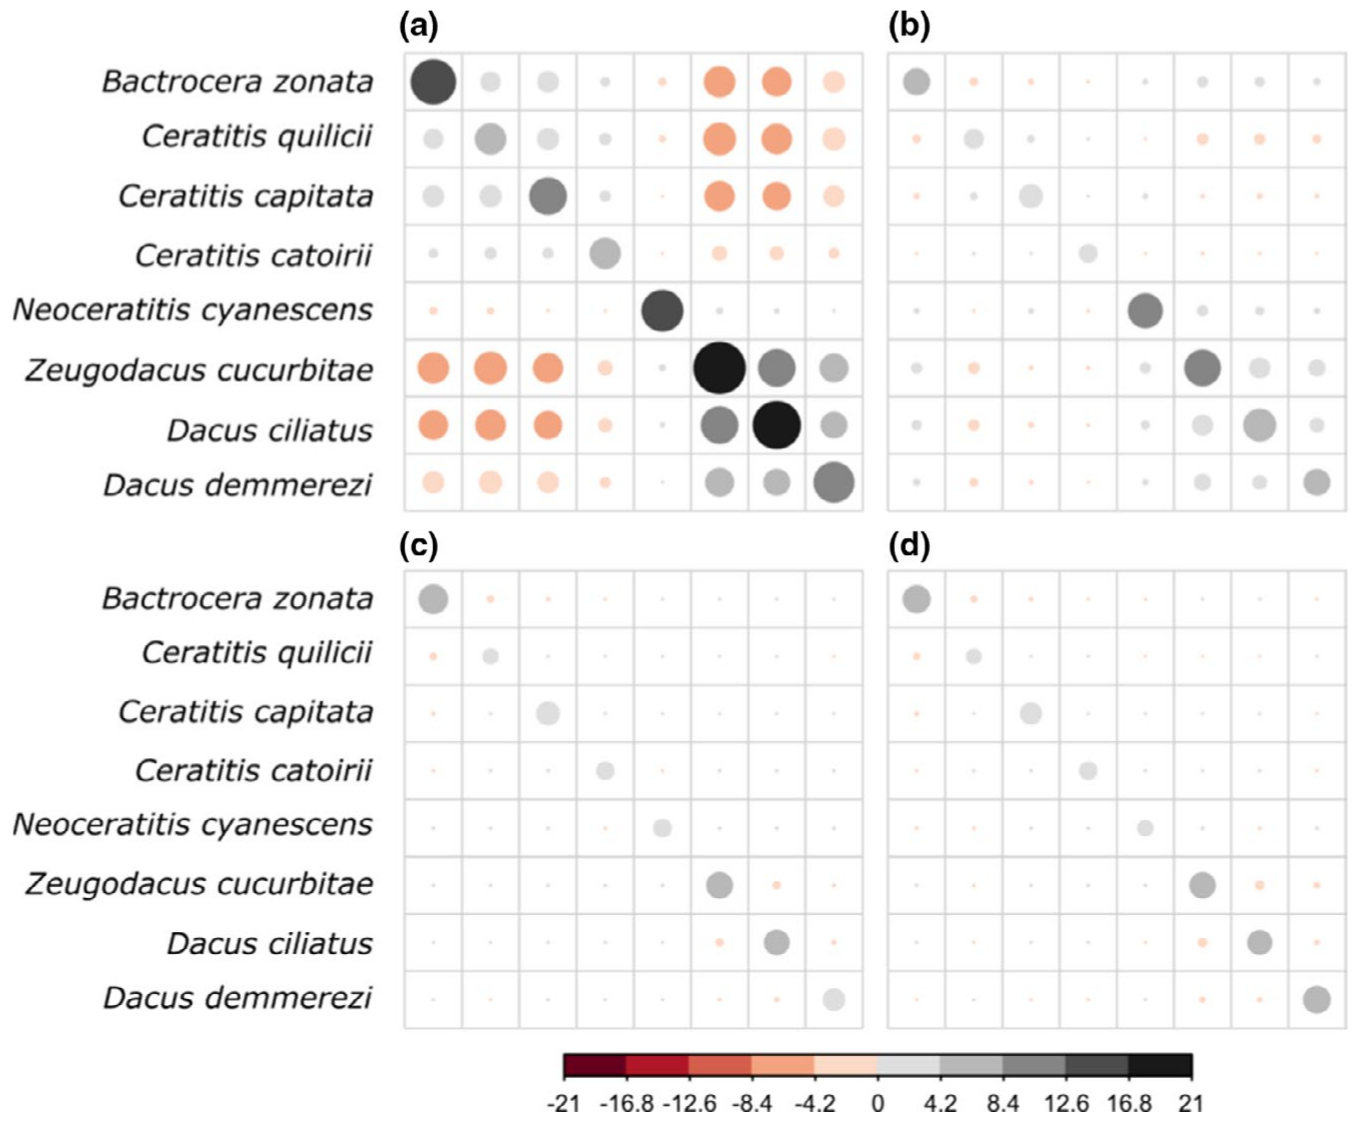
\includegraphics[width=.5\textwidth]{\figeco/FHC20-EcolLetters-Fig2}
  $$
  $$
  \begin{tabular}{clcl}
    \qquad & (a) No covariate & \qquad \qquad & (b) Climat \\
    \qquad & (c) Plant species & & (d) Plant species and climat
  \end{tabular}
  $$
  
  \bigskip
  \ra Weak competition among species specialists of the same plant.
}



%====================================================================
\subsection{Dimension reduction}
%====================================================================
\frame{\frametitle{Dimension reduction (PCA)} \pause

  \paragraph{Dimension reduction.} 
  \begin{itemize}
    \setlength{\itemsep}{0.5\baselineskip}
  \item Metagenomic, metabarcoding, environmental genomics: $p = 10^2, 10^3$ species.
  \item (Probabilistic) PCA \refer{Tib99}: the latent dimension of the data is actually $q \ll p$.
  \end{itemize}
  
  \pause \bigskip \bigskip 
  \paragraph{PLN-PCA model = reduced latent dimension.}  \refer{CMR18a}
  \begin{itemize}
    \setlength{\itemsep}{0.5\baselineskip}
    \item Do not need a latent vector $Z_i$ with $p$ free coordinates in each site. 
    \item \pause A latent vector $W_i$ with $q \ll p$ free coordinates suffices:
    $$
    W_i = [W_{i1} \; \dots \; W_{iq}] \sim \Ncal(0, I_q).
    $$ 
    \item \pause $Z_i$ can then be reconstructed from $W_i$ as $Z_i = B W_i$, where $B: p \times q$.
  \end{itemize}

  \pause \bigskip
  \ra The covariance matrix $\Sigma$ has rank $q \ll p$: 'low-rank' approximation.
  
  \pause \bigskip \bigskip 
  \paragraph{Model selection.} The latent dimension $q$ can be selected using standard criteria (BIC, ICL, ...).

}

%====================================================================
\frame{\frametitle{Oak powdery mildew dataset (1/2)}

  \bigskip 
  \paragraph{Metabarcoding data.} \refer{JFS16} 
  \begin{itemize}
    \setlength{\itemsep}{1\baselineskip}
    \item $p = 114$ OTUs (bacteria and fungi) \\ 
      \ra different extraction protocol for each group.
    \item $n = 116$ leaves = samples \\
      \ra collected from 3 different trees, at different positions in the tree.
    \item $Y_{ij} =$ read count for species $j$ in sample $i$.
  \end{itemize}
  
  \pause \bigskip \bigskip 
  \paragraph{Questions.}
  \begin{itemize}
    \setlength{\itemsep}{0.5\baselineskip}
    \item Effect of the covariates (tree, position) on the abundance of the species.
    \item Visualization.
    \item Account for the heterogeneity of the sampling protocol.
  \end{itemize}

  \pause \bigskip \bigskip 
  \paragraph{Use of the offset.}
  $$
  o_{ij} = \log(\text{total sequencing depth of sample $i$ for the group of species $j$}).
  $$
}

%====================================================================
\frame{\frametitle{Oak powdery mildew dataset (2/2)}

  $$
  \begin{tabular}{c}
    \includegraphics[height=.38\textheight]{\fignet/CMR18-AnnApplStat-Fig4a} \\
    \pause ~ % \\
    \includegraphics[height=.38\textheight]{\fignet/CMR18-AnnApplStat-Fig5a} 
  \end{tabular}
  $$
  \pause
  \ra Other main effects = distance to the ground, then orientation. 
}

%====================================================================
\frame{\frametitle{Microbiote of young pigs}

  \paragraph{Data.} \refer{MBE15}
  \begin{itemize}
    \item $n = 155$ piglets, 
    \item $p = 500$ OTUs ($= 90\%$ of the total abundance of the original 4031 OTU)
  \end{itemize}
  
  \pause \bigskip \bigskip 
  \paragraph{Question.} 
  Effect of weaning

  \pause \bigskip \bigskip 
  \paragraph{PLN-PCA.} No covariate:
  $$
  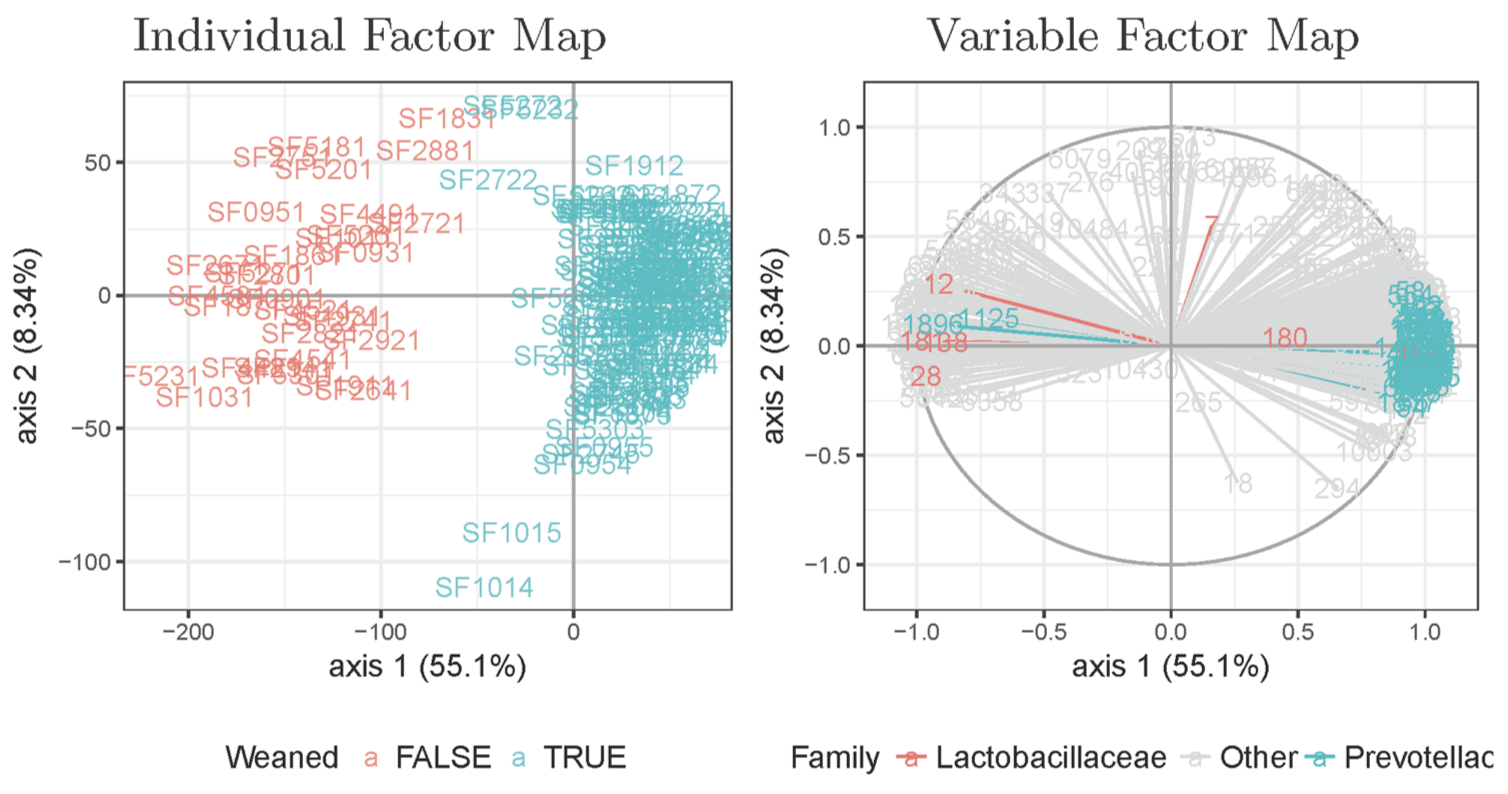
\includegraphics[height=.45\textheight]{\figeco/CMR18-AnnApplStat-Fig3}
  $$  

}



%====================================================================
\subsection{Network inference}
%====================================================================
\frame{\frametitle{Network inference} \pause

  \bigskip
  \paragraph{Distinguishing between direct and indirect interactions.}
  \begin{itemize}
    \setlength{\itemsep}{0.5\baselineskip}
    \item The variations of species abundance can be all correlated,
    \item Some correlations result from 'direct' interactions ($A$ eats $B$). 
    \item Some others result from 'indirect' interactions  (both $A$ and $B$ are preys of $C$).
  \end{itemize}
   \pause \medskip
  \ra Probabilistic translation: \emphase{\sl conditional} dependence vs \emphase{\sl marginal} dependence.

  \pause \bigskip \bigskip
  \paragraph{Graphical model} encodes the dependency structure into a graph $G$ in which only conditionally {\sl dependent variables} are connected.
  
  \pause \bigskip \bigskip \bigskip
  \begin{tabular}{cc}
    \hspace{-.04\textwidth}
    \begin{tabular}{p{.65\textwidth}}
      \paragraph{Example:}
      \begin{itemize}
        \setlength{\itemsep}{0.5\baselineskip}
        \item All variables (species) are dependent
        \item But 4 is independent from 1 and 2 conditionally on 3 \\ ~
        \item \textcolor{gray}{Formally: $p(y_1, y_2, y_3, y_4) \propto \psi_1(y_1, y_2, y_3) \psi_2(y_3, y_4).$}
      \end{itemize}
      \bigskip \bigskip ~
    \end{tabular}
    &
    \begin{tabular}{p{.25\textwidth}}
      \hspace{-.1\textwidth}
      \includegraphics[width=.3\textwidth, trim=90 90 50 90, clip=]{\fignet/FigGGM-4nodes}
    \end{tabular}
  \end{tabular}

}

%====================================================================
\frame{\frametitle{Network inference in the PLN model} \pause

  \bigskip
  \paragraph{PLN model.} The dependency is encoded in the Gaussian latent layer, with covariance matrix $\Sigma$.
  
  \pause \bigskip \bigskip
  \paragraph{Gaussian case.} The graph $G$ of direct interactions is given by the precision matrix
  $$
  \Omega = \Sigma^{-1}
  $$
  ({\sl partial} correlations vs {\sl marginal} correlations).
  
  \pause \bigskip \bigskip \bigskip 
  \begin{tabular}{cc}
    \hspace{-.04\textwidth}
    \begin{tabular}{p{.6\textwidth}}
      \paragraph{PLN version.} \refer{CMR19}
      \medskip
      \begin{itemize}
        \setlength{\itemsep}{1\baselineskip}
        \item Fit a PLN model, forcing $\Omega = \Sigma^{-1}$ to be sparse.
        \item Algorithm similar to the graphical lasso \refer{FHT08}. \\ ~
        \item \pause The sparsity of $\Omega$ is tuned via a penalty parameter $\lambda$.
        \item $\lambda$ can be chosen via standard criteria (BIC, ...).
      \end{itemize}
      \bigskip \bigskip ~
    \end{tabular}
    &
    \hspace{-.05\textwidth}
    \begin{tabular}{p{.4\textwidth}}
      \includegraphics[height=.5\textheight, trim=25 5 10 0, clip=]{\fignet/BarentsFish_Gfull_criteria}
    \end{tabular}
  \end{tabular}

}

%====================================================================
\frame{\frametitle{Barents' fish} 
  
  \vspace{-.05\textheight}
  \begin{tabular}{cc}
    \hspace{-.04\textwidth}
    \begin{tabular}{p{.22\textwidth}}
      \paragraph{Data:} \\ ~
      \begin{itemize}
      \item $n=89$ sites \\~
      \item $p=30$ species \\~
      \item $d=4$ covariates
        \begin{itemize}
        \item latitude
        \item longitude
        \item temperature
        \item depth
        \end{itemize}
      \end{itemize}
    \end{tabular}
    &
    \begin{tabular}{c}
      \includegraphics[height=.85\textheight]{\fignet/CMR18b-ArXiv-Fig5}
    \end{tabular}
  \end{tabular}
  }

%====================================================================
\frame{\frametitle{Oak powdery mildew}

  \begin{tabular}{cc}
    \hspace{-.04\textwidth}
    \begin{tabular}{p{.35\textwidth}}
      \paragraph{Network inference.} \refer{JFS16} ~
      
      \bigskip
      {\sl Erysiphe alphitoides} (Ea) = \\
      ~ \\
      fungus reponsible for the disease
    \end{tabular}
    &
%     \hspace{-.075\textwidth}
    \begin{tabular}{p{.65\textwidth}}
      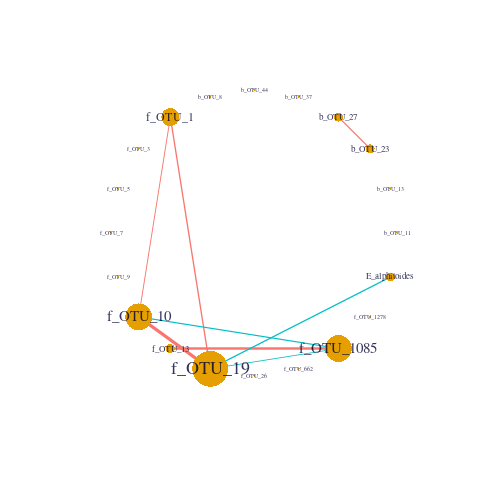
\includegraphics[height=.7\textheight, trim=50 50 50 50, clip=]{\fignet/Oaks-p20-network}
    \end{tabular}
  \end{tabular}

  
  \pause \bigskip
  \ra See also tree-based network inference, including {\sl missing actors} \refer{SRS19,MRA20,MRA21}
}



%====================================================================
\subsection{Zero inflation}
%====================================================================
\frame{\frametitle{Zero inflation} \pause

  \todo{TO DO}
}





%====================================================================
%====================================================================
\section{Conclusion}
%====================================================================
\frame{\frametitle{Conclusion} 

  \paragraph{Poisson log-normal model.} \refer{CMR20}
  \begin{itemize}
    \setlength{\itemsep}{1\baselineskip}
    \item Flexible modeling framework for multivariate abundance data.
    \item \pause Other avatars: sample classification, sample clustering, ...
    \item \pause Implemented in the \emphase{R package \url{PLNmodels}} .
    \item \pause Jackknife estimates of the variances (with computational cost).
  \end{itemize}

  \pause \bigskip \bigskip 
  \paragraph{On-going works:}
  \begin{itemize}
    \setlength{\itemsep}{1\baselineskip}
    \item Include species traits.
    \item Account for dependence between sites (or samples).
    \item 'Zero-inflated' version.
    \item Monte-Carlo E step to achieve maximum (composite) likelihood.
  \end{itemize}

}
  


%====================================================================
%====================================================================
\backupbegin 
\section*{Backup}
%====================================================================
\frame[allowframebreaks]{ \frametitle{References}
  {%\footnotesize
   \tiny
   \bibliography{/home/robin/Biblio/BibGene}
%    \bibliographystyle{/home/robin/LATEX/Biblio/astats}
   \bibliographystyle{alpha}
  }
}

%====================================================================
\frame{\frametitle{Microbiote of young pigs}

  \paragraph{Effect of species selection.} 
  $$
  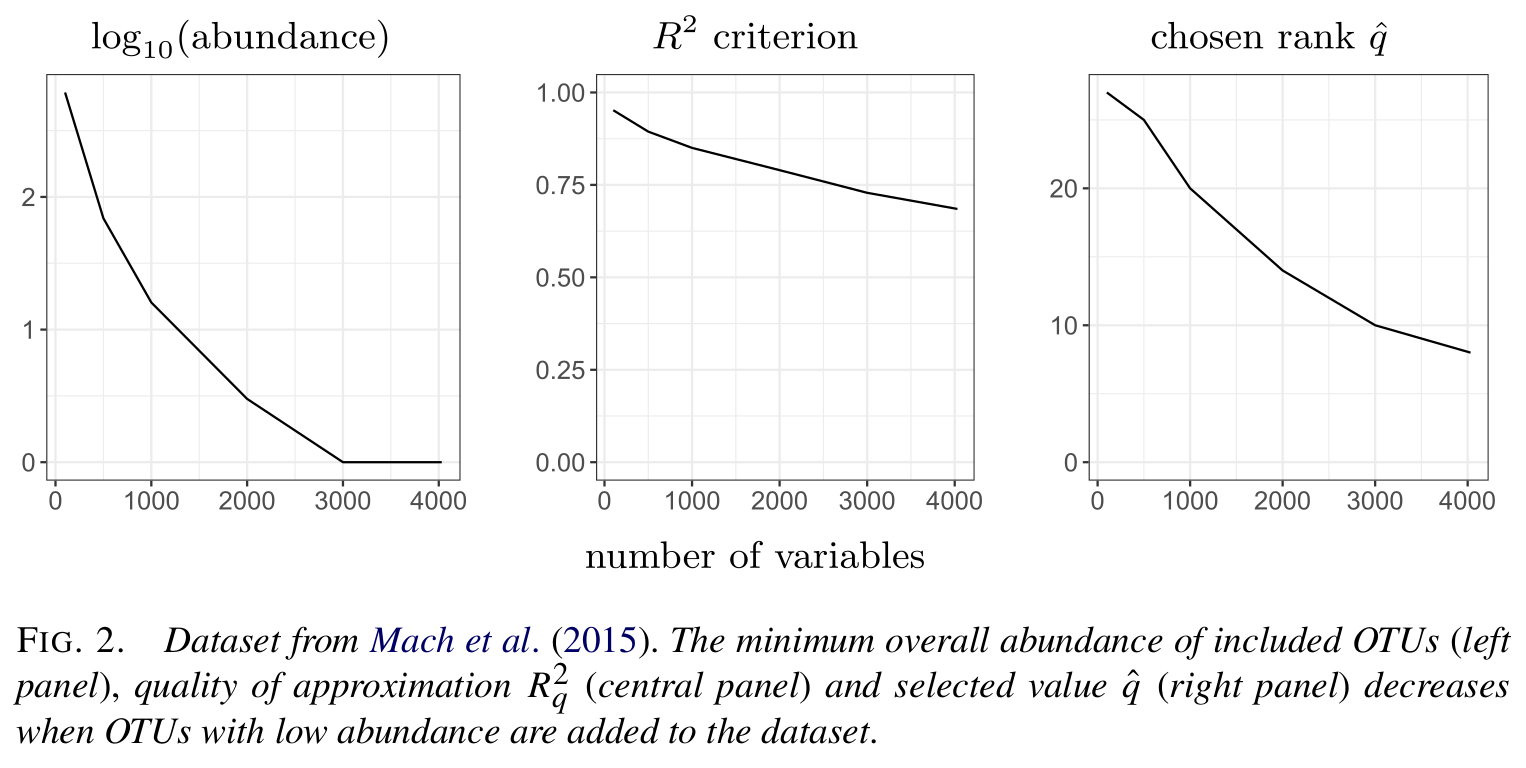
\includegraphics[height=.6\textheight]{\figeco/CMR18-AnnApplStat-Fig2}
  $$  

}

%====================================================================
\frame{\frametitle{Oak powdery mildew}

  \paragraph{Tree-specific network inference.}
  $$
  \begin{tabular}{ccc}
    susceptible & intermediate & resistant \\
    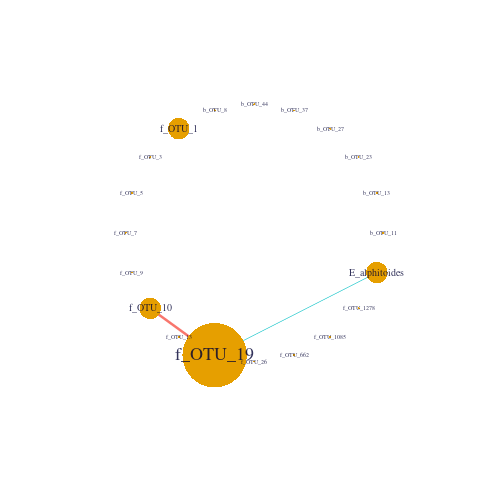
\includegraphics[height=.42\textheight, trim=70 70 70 70, clip=]{\fignet/Oaks-p20-network-susceptible} &
    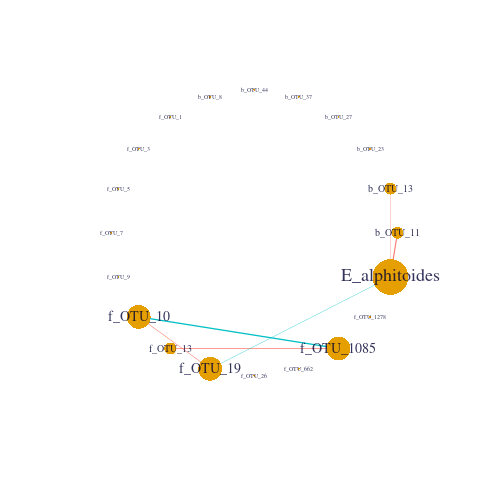
\includegraphics[height=.42\textheight, trim=70 70 70 70, clip=]{\fignet/Oaks-p20-network-intermediate} &
    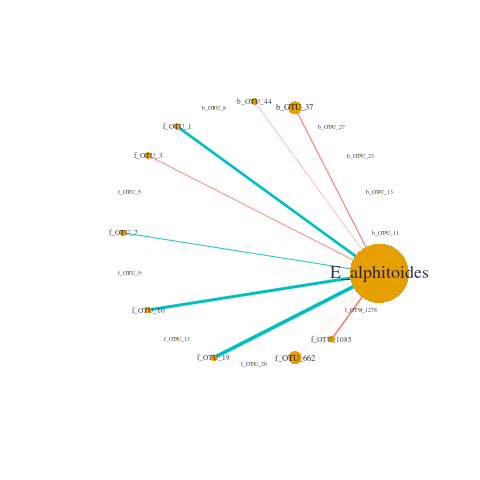
\includegraphics[height=.42\textheight, trim=70 70 70 70, clip=]{\fignet/Oaks-p20-network-resistant}
  \end{tabular}
  $$
}

%====================================================================
\backupend 



%====================================================================
%====================================================================
\end{document}
%====================================================================
%====================================================================

  \begin{tabular}{cc}
    \hspace{-.04\textwidth}
    \begin{tabular}{p{.5\textwidth}}
    \end{tabular}
    &
    \begin{tabular}{p{.45\textwidth}}
    \end{tabular}
  \end{tabular}

